\documentclass[11pt,a4paper]{article}

\usepackage[headsep=1cm,headheight=3cm,left=3.5cm,right=3.5cm,top=2.5cm,bottom=2.5cm,a4paper]{geometry}

\linespread{1.3}
\setlength{\parindent}{0pt}
\setlength{\parskip}{1em}

\usepackage[spanish]{babel}
\usepackage[utf8]{inputenc}

%% Fuentes personalizadas para utilizar con XeTeX
\usepackage[sfdefault]{roboto}
\usepackage[scaled=0.9]{DejaVuSansMono}
\usepackage[T1]{fontenc}

\usepackage{enumitem}
\setlist[itemize]{leftmargin=*}
\setlist[enumerate]{leftmargin=*}

\usepackage{changepage}

\newcounter{ActCounter}
\newcommand{\act}[1]{\addtocounter{ActCounter}{1}\textbf{\sffamily ACT-\theActCounter}\quad#1\\}

\newcounter{CUCounter}
\newcommand{\cu}[1]{\addtocounter{CUCounter}{1}\textbf{\sffamily CU-\theCUCounter}\quad#1\\}

\usepackage{tabularx}
\usepackage{float}
\usepackage{adjustbox}

\title{Práctica 2: Modelo de casos de uso \large\\ Fundamentos de Ingeniería del Software}
\author{Sofía Almedia Bruno \and José Antonio Álvarez Ocete \and Miguel Lentisco Ballesteros \and Simón López Vico \and José María Martín Luque}

\begin{document}

\maketitle

\section{Introducción}

En el presente documento se muestra el modelo de Casos de Uso obtenido en el proceso de análisis del sistema para la gestión de un centro médico. El modelo se puede descomponer en dos grandes paquetes que agrupan las funcionalidades básicas del sistema.

\section{Diagramas de casos de uso} % (fold)

\begin{figure}[H]
	\caption{Diagrama de casos de uso de gestión de datos}
	\centering
	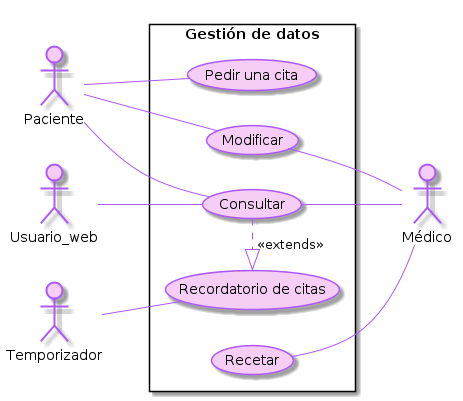
\includegraphics{diagramas/gestion_datos}
\end{figure}

\begin{figure}[H]
	\caption{Diagrama de casos de uso de contabilidad}
	\centering
	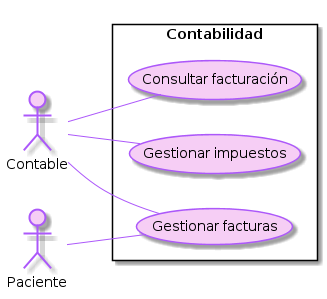
\includegraphics{diagramas/contabilidad}
\end{figure}

\section{Descripción de los actores}
% PLANTILLA PACIENTE

\begin{table}[H]
\label{my-label}
\begin{tabularx}{\textwidth}{l|Xlllr}
	\textbf{Actor}           & \multicolumn{4}{l}{Paciente} & \act\\ 
	\textbf{Descripción}     & \multicolumn{5}{>{\hsize=\dimexpr\textwidth-\hsize\relax}X}{Paciente adscrito al centro médico que desea pedir cita, consultar su historial o informarse acerca de la clínica}\\
	\textbf{Características} & \multicolumn{5}{>{\hsize=2\hsize}X}{Todos los clientes de la clínica son pacientes}\\ 
	\textbf{Relaciones}      & \multicolumn{5}{>{\hsize=2\hsize}X}{No tiene}\\ 
	\textbf{Referencias}     & \multicolumn{5}{>{\hsize=2\hsize}X}{Pedir una cita, modificar, consultar}\\
	\textbf{Autor}           & Grupo ? & \textbf{Fecha} & 07/04/18 & \textbf{Versión} & {1.1}                      \\ 
\end{tabularx}
\end{table}

\begin{table}[H]
\label{my-label}
\begin{tabularx}{\textwidth}{lXl}
	\textbf{Atributos} &  & \\
	\textbf{Nombre}    & \textbf{Descripción} & \textbf{Tipo} \\ \hline
	Datos personales   & Identifican al paciente (\texttt{Id\_paciente}, DNI, nombre y apellidos, ...)     & \\
	Contacto           & Permiten ponerse en contacto con el paciente o algún familiar (teléfono, en caso de emergencia avisar a ...) & \\  
	Datos médicos      & Información relativa a la salud del paciente (historial médico, grupo sanguíneo, enfermedades previas, alergias, ...)            
\end{tabularx}
\end{table}

\begin{table}[H]
\begin{tabularx}{\textwidth}{X}
	\textbf{Comentarios}\\ \hline
\end{tabularx}
\end{table}
% FIN PLANTILLA PACIENTE

\newpage

% PLANTILLA MÉDICO

\begin{table}[H]
\label{my-label}
\begin{tabularx}{\textwidth}{l|Xlllr}
	\textbf{Actor}           & Médico & & & & \act \\ 
	\textbf{Descripción}     & \multicolumn{5}{>{\hsize=\dimexpr\textwidth-\hsize\relax}X}{Personal sanitario de la clínica}\\
	\textbf{Características} & \multicolumn{5}{>{\hsize=\dimexpr\textwidth-\hsize\relax}X}{Puede modificar la información del paciente}\\ 
	\textbf{Relaciones}      & \multicolumn{5}{>{\hsize=\dimexpr\textwidth-\hsize\relax}X}{}\\ 
	\textbf{Referencias}     & \multicolumn{5}{>{\hsize=\dimexpr\textwidth-\hsize\relax}X}{}\\ 
	\textbf{Autor}           &  & \textbf{Fecha} & & \textbf{Versión} & \\ 
\end{tabularx}
\end{table}

\begin{table}[H]
\label{my-label}
\begin{tabularx}{\textwidth}{lXl}
	\textbf{Atributos} &  & \\
	\textbf{Nombre}    & \textbf{Descripción} & \textbf{Tipo} \\ \hline
	Datos personales   &  Identifican al médico (\texttt{Id\_médico}, DNI, nombre y apellidos,...)     & \\
	Datos laborales    & Relativos a su trabajo (horario, sueldo, vacaciones,...) &
\end{tabularx}
\end{table}

\begin{table}[H]
\begin{tabularx}{\textwidth}{X}
	\textbf{Comentarios}\\ \hline
\end{tabularx}
\end{table}

% FIN PLANTILLA MÉDICO

\newpage

% PLANTILLA CONTABLE

\begin{table}[H]
	\label{my-label}
	\begin{tabularx}{\textwidth}{l|Xlllr}
		\textbf{Actor}           & \multicolumn{4}{l}{Contable} & \act\\ 
		\textbf{Descripción}     & \multicolumn{5}{>{\hsize=\dimexpr\textwidth-\hsize\relax}X}{Encargado de gestionar la facturación y los impuestos referentes a la clínica.}\\
		\textbf{Características} & \multicolumn{5}{>{\hsize=\dimexpr\textwidth-\hsize\relax}X}{Puede consultar las facturas de todo cliente en el sistema y el sueldo del personal, así como etiquetar como moroso a aquel cliente que debe dinero.}\\ 
		\textbf{Relaciones}      & \multicolumn{5}{>{\hsize=\dimexpr\textwidth-\hsize\relax}X}{Paciente, personal.}\\ 
		\textbf{Referencias}     & \multicolumn{5}{>{\hsize=\dimexpr\textwidth-\hsize\relax}X}{Consultar facturación, gestionar impuestos, gestionar facturas.}\\
		\textbf{Autor}           & Simón López & \textbf{Fecha} & 04/04/18 & \textbf{Versión} & \textbf{1.0}                      \\ 
	\end{tabularx}
\end{table}

\begin{table}[H]
	\label{my-label}
	\begin{tabularx}{\textwidth}{lXl}
		\textbf{Atributos}  &  & \\
		\textbf{Nombre}     & \textbf{Descripción} & \textbf{Tipo} \\ \hline
		\textbf{IdContable} & Nombre o pseudónimo referente al contable, único en el sistema que identificará a este. & Texto \\
		\textbf{Salario}    & Cantidad de dinero que cobra el contable al mes. & Numérico \\
	\end{tabularx}
\end{table}

\begin{table}[H]
	\begin{tabularx}{\textwidth}{X}
		\textbf{Comentarios}\\ \hline
		Usualmente no habrá más de un contable por clínica.
	\end{tabularx}
\end{table}

%FIN DE LA PLANTILLA CONTABLE

\newpage

% PLANTILLA USUARIO WEB

\begin{table}[H]
	\label{my-label}
	\begin{tabularx}{\textwidth}{l|Xlllr}
		\textbf{Actor}           & \multicolumn{4}{l}{Usuario web} & \act\\ 
		\textbf{Descripción}     & \multicolumn{5}{>{\hsize=\dimexpr\textwidth-\hsize\relax}X}{Cualquier persona que acceda a la información disponible en la página web}\\
		\textbf{Características} & \multicolumn{5}{>{\hsize=\dimexpr\textwidth-\hsize\relax}X}{Puede acceder a diversa información tal como las especialidades, tratamientos, horarios, instalaciones o médicos disponibles.}\\ 
		\textbf{Relaciones}      & \multicolumn{5}{>{\hsize=\dimexpr\textwidth-\hsize\relax}X}{No tiene.}\\ 
		\textbf{Referencias}     & \multicolumn{5}{>{\hsize=\dimexpr\textwidth-\hsize\relax}X}{}\\
		\textbf{Autor}           & Miguel Lentisco & \textbf{Fecha} & 04/04/18 & \textbf{Versión} & \textbf{1.0}                      \\ 
	\end{tabularx}
\end{table}

\begin{table}[H]
	\begin{tabularx}{\textwidth}{X}
		\textbf{Comentarios}\\\hline
		No se va a guardar información sobre estos usuarios, puede ser cualquier persona que quiera informarse sobre la clínica
	\end{tabularx}
\end{table}

% FIN DE LA PLANTILLA USUARIO WEB

\newpage

% PLANTILLA TEMPORIZADOR

\begin{table}[H]
	\label{my-label}
	\begin{tabularx}{\textwidth}{l|Xlllr}
		\textbf{Actor}           & \multicolumn{4}{l}{Temporizador} & \act\\ 
		\textbf{Descripción}     & \multicolumn{5}{>{\hsize=\dimexpr\textwidth-\hsize\relax}X}{Daemon cuyo objetivo es recordar las citas a los demas usuarios del sistema}\\
		\textbf{Características} & \multicolumn{5}{>{\hsize=\dimexpr\textwidth-\hsize\relax}X}{Accede a los horarios de los distintos usuarios del sistema de forma periódica y avisa tanto a clientes como a trabajadores de su horario.}\\ 
		\textbf{Relaciones}      & \multicolumn{5}{>{\hsize=\dimexpr\textwidth-\hsize\relax}X}{No tiene.}\\ 
		\textbf{Referencias}     & \multicolumn{5}{>{\hsize=\dimexpr\textwidth-\hsize\relax}X}{}\\
		\textbf{Autor}           & José Antonio Álvarez & \textbf{Fecha} & 05/04/18 & \textbf{Versión} & \textbf{1.0}                      \\ 
	\end{tabularx}
\end{table}

\begin{table}[H]
	\begin{tabularx}{\textwidth}{X}
		\textbf{Comentarios}\\ \hline
		Sobre este actor tampoco se almacenan información debido a sus funcionalidades
	\end{tabularx}
\end{table}

% FIN DE LA PLANTILLA TEMPORIZADOR

\newpage

\section{Descripción de los casos de uso}

% PEDIR CITA

\begin{table}[H]
	\begin{tabularx}{\textwidth}{l|Xlllr}
		\textbf{Caso de Uso}   & Pedir cita & & & & \cu \\  
		\textbf{Actores}       & Paciente & & & \\ 
		\textbf{Tipo}          & Primario & & & \\
		\textbf{Referencias}   & RF-1, RN-1, RN-2, RI-1 & & & \\
		\textbf{Precondición}  & \multicolumn{5}{>{\hsize=\dimexpr\textwidth-0.85\hsize\relax}X}{Plataforma activa y operativa, paciente correctamente identificado}\\ 
		\textbf{Postcondición} & Cita añadida al sistema & & & & \\
		\textbf{Autor}         & Grupo ? & \textbf{Fecha} & 07/04/18 & \textbf{Versión} & 1.0 \\ 
	\end{tabularx}
\end{table}

\begin{table}[H]
	\begin{tabularx}{\textwidth}{X}
		\textbf{Propósito}\\ \hline
		Permitir que un paciente reserve una cita con su médico
	\end{tabularx}
\end{table}

\begin{table}[H]
	\begin{tabularx}{\textwidth}{X}
		\textbf{Resumen}\\ \hline
		Tras la identificación del paciente éste podrá observar en qué fecha y horario su médico tiene citas disponibles y seleccionar una de ellas, el sistema la marcará como reservada por este paciente.
	\end{tabularx}
\end{table}

% FIN PEDIR CITA

\newpage

% MODIFICAR

\begin{table}[H]
	\begin{tabularx}{\textwidth}{l|Xlllr}
		\textbf{Caso de Uso}   & Modificar & & & & \cu \\  
		\textbf{Actores}       & Paciente, médico & & & \\ 
		\textbf{Tipo}          & Secundario, esencial & & & \\
		\textbf{Referencias}   & \multicolumn{5}{>{\hsize=\dimexpr\textwidth-\hsize\relax}X}{RF-2, RF-9, RF-13, RF-15, RNF-1, RNF-2}\\
		\textbf{Precondición}  & \multicolumn{5}{>{\hsize=\dimexpr\textwidth-0.85\hsize\relax}X}{Plataforma activa y operativa, usuario y/o médico registrados en el sistema.}\\ 
		\textbf{Postcondición} & - & & & & \\
		\textbf{Autor}         & Grupo ? & \textbf{Fecha} & 05/04/18 & \textbf{Versión} & 1.0 \\ 
	\end{tabularx}
\end{table}

\begin{table}[H]
	\begin{tabularx}{\textwidth}{X}
		\textbf{Propósito}\\ \hline
		Dar la posibilidad de modificar los datos sobre un elemento del sistema tras haberlos introducido en su registro
	\end{tabularx}
\end{table}

\begin{table}[H]
	\begin{tabularx}{\textwidth}{X}
		\textbf{Resumen}\\ \hline
		El usuario accede a su ficha médica (o el médico a la de éste) y solicita modificar sus datos, introduciendo los nuevos y aceptando la modificación de éstos. También pueden modificarse las listas de espera y el horario de los médicos de manera similar
	\end{tabularx}
\end{table}

% FIN DE MODIFICAR

\newpage

% INICIO DE RECETAR

\begin{table}[H]
	\begin{tabularx}{\textwidth}{l|Xlllr}
		\textbf{Caso de Uso}   & Modificar & & & & \cu \\  
		\textbf{Actores}       & Paciente, médico & & & \\ 
		\textbf{Tipo}          & Primario, esencial & & & \\
		\textbf{Referencias}   & \multicolumn{5}{>{\hsize=\dimexpr\textwidth-\hsize\relax}X}{RF-12, Consultar}\\
		\textbf{Precondición}  & \multicolumn{5}{>{\hsize=\dimexpr\textwidth-0.85\hsize\relax}X}{Plataforma activa y operativa, usuario y médico registrados en el sistema}\\ 
		\textbf{Postcondición} & \multicolumn{5}{>{\hsize=\dimexpr\textwidth-0.85\hsize\relax}X}{Historial médico correctamente modificado}\\
		\textbf{Autor}         & Grupo ? & \textbf{Fecha} & 05/04/18 & \textbf{Versión} & 1.0 \\ 
	\end{tabularx}
\end{table}

\begin{table}[H]
	\begin{tabularx}{\textwidth}{X}
		\textbf{Propósito}\\ \hline
		El médico receta al paciente las medicinas que necesite (añadidas al historial médico)
	\end{tabularx}
\end{table}

\begin{table}[H]
	\begin{tabularx}{\textwidth}{X}
		\textbf{Resumen}\\ \hline
		Seleccionado el paciente al que se le va a recetar, el médico solicita ver la lista de recetas disponibles poniendo un filtro adecuado si lo cree necesario (como por nombre, tipo...). El sistema le devuelve la lista de medicamentos disponibles, y el médico selecciona las recetas oportunas, entonces estas se cargan al historial médico del paciente
	\end{tabularx}
\end{table}

% FIN RECETAR

\newpage

% INICIO DE GESTIÓN DE IMPUESTOS

\begin{table}[H]
	\begin{tabularx}{\textwidth}{l|Xlllr}
		\textbf{Caso de Uso}   & Gestionar impuestos & & & & \cu \\  
		\textbf{Actores}       & Contable & & & \\ 
		\textbf{Tipo}          & Primario, esencial & & & \\
		\textbf{Referencias}   & \multicolumn{5}{>{\hsize=\dimexpr\textwidth-\hsize\relax}X}{RF-25, RNF-1, Consultar}\\
		\textbf{Precondición}  & \multicolumn{5}{>{\hsize=\dimexpr\textwidth-0.85\hsize\relax}X}{Plataforma activa y operativa, acceso al sistema con una usuario contable para gestionar los impuestos}\\ 
		\textbf{Postcondición} & \multicolumn{5}{>{\hsize=\dimexpr\textwidth-0.85\hsize\relax}X}{Notificar al gerente de la modificación de la contabilidad en la clínica}\\
		\textbf{Autor}         & Grupo ? & \textbf{Fecha} & 06/04/18 & \textbf{Versión} & 1.0 \\ 
	\end{tabularx}
\end{table}

\begin{table}[H]
	\begin{tabularx}{\textwidth}{X}
		\textbf{Propósito}\\ \hline
		Facilitar al contable la gestión de los impuestos referente a la clínica, pudiendo gestionar la contabilidad mediante el sistema informático
	\end{tabularx}
\end{table}

\begin{table}[H]
	\begin{tabularx}{\textwidth}{X}
		\textbf{Resumen}\\ \hline
		El contable entra al sistema mediante su cuenta de contable y accede al apartado de gestión de impuestos, donde podrá dividir el dinero de la clínica en los distintos apartados posibles (investigación, compra de material...). Tras esto, se enviará una notificación al gerente de que se han modificado las cuentas del hospital
	\end{tabularx}
\end{table}

% FIN DE GESTIÓN DE IMPUESTOS

\newpage

% INICIO CONSULTAR FACTURACION

\begin{table}[H]
	\begin{tabularx}{\textwidth}{l|Xlllr}
		\textbf{Caso de Uso}   & Consultar facturación & & & & \cu \\  
		\textbf{Actores}       & Contable & & & \\ 
		\textbf{Tipo}          & Opcional, esencial & & & \\
		\textbf{Referencias}   & \multicolumn{5}{>{\hsize=\dimexpr\textwidth-\hsize\relax}X}{RF-5, RF-24, RF-26}\\
		\textbf{Precondición}  & \multicolumn{5}{>{\hsize=\dimexpr\textwidth-0.85\hsize\relax}X}{Plataforma activa y operativa}\\ 
		\textbf{Postcondición} & \multicolumn{5}{>{\hsize=\dimexpr\textwidth-0.85\hsize\relax}X}{-}\\
		\textbf{Autor}         & Grupo ? & \textbf{Fecha} & 06/04/18 & \textbf{Versión} & 1.0 \\ 
	\end{tabularx}
\end{table}

\begin{table}[H]
	\begin{tabularx}{\textwidth}{X}
		\textbf{Propósito}\\ \hline
		Visualizar la facturación de la clínica y las tareas en las que se ha invertido el dinero de ésta
	\end{tabularx}
\end{table}

\begin{table}[H]
	\begin{tabularx}{\textwidth}{X}
		\textbf{Resumen}\\ \hline
		El contable entra al sistema mediante su cuenta de contable y accede al apartado consultar facturación, donde aparecerán distintas tablas con la facturación referente a la clínica
	\end{tabularx}
\end{table}

% FIN CONSULTAR FACTURACIÓN

\newpage

% INICIO DE GESTIONAR FACTURAS

\begin{table}[H]
	\begin{tabularx}{\textwidth}{l|Xlllr}
		\textbf{Caso de Uso}   & Gestionar facturas & & & & \cu \\  
		\textbf{Actores}       & Contable, paciente & & & \\ 
		\textbf{Tipo}          & Primario, esencial & & & \\
		\textbf{Referencias}   & \multicolumn{5}{>{\hsize=\dimexpr\textwidth-\hsize\relax}X}{RF-5, RF-24, RF-26, RNF-1}\\
		\textbf{Precondición}  & \multicolumn{5}{>{\hsize=\dimexpr\textwidth-0.85\hsize\relax}X}{Plataforma activa y operativa, factura a la que se quiere acceder registrada en el sistema}\\ 
		\textbf{Postcondición} & \multicolumn{5}{>{\hsize=\dimexpr\textwidth-0.85\hsize\relax}X}{Facturas correctamente modificadas. En caso de que el contable etiquete como moroso a un paciente por no haber pagado, notificar al paciente}\\
		\textbf{Autor}         & Grupo ? & \textbf{Fecha} & 06/04/18 & \textbf{Versión} & 1.0 \\ 
	\end{tabularx}
\end{table}

\begin{table}[H]
	\begin{tabularx}{\textwidth}{X}
		\textbf{Propósito}\\ \hline
		Dar la opción al paciente para que gestione su seguro médico referente a la clínica mediante el sistema informático, haciendo que no se tenga que desplazar a la clínica para gestionar sus facturas. Por parte del contable, gestionar las distintas facturas de cada paciente para comprobar que todas están pagadas y bien establecidas
	\end{tabularx}
\end{table}

\begin{table}[H]
	\begin{tabularx}{\textwidth}{X}
		\textbf{Resumen}\\ \hline
		El paciente o el contable acceden al sistema mediante su usuario y seleccionan el apartado gestionar facturas, donde aparecerán sus facturas ordenadas junto a distintas opciones a realizar sobre ellas. El contable podrá hacer una búsqueda sobre todas las facturas del sistema y gestionar la de cualquier paciente
	\end{tabularx}
\end{table}

% FIN DE GESTIONAR FACTURAS

\newpage

% TODO: CAMBIAR esto, sorry por el formato
\begin{itemize}
	\item Médico: selección del recetario
	\item Médico: uso de filtro de búsqueda
	\item Sistema: devuelve lista de recetas disponibles válidas
	\item Médico: selección de recetas
	\item Sistema: recetas añadidas al historial médico
\end{itemize}


\begin{itemize}
	\item Frecuencia esperada: una por cita.
	\item Importancia: baja
	\item Estado: sin implementar
	\item Rendimiento: alto
	\item Urgencia: baja
	\item Estabilidad: alta
\end{itemize}


% FIN DE RECETAR

\newpage
\section{Diagrama de paquetes}

\begin{figure}[H]
	\caption{Diagrama de paquetes}
	\centering
	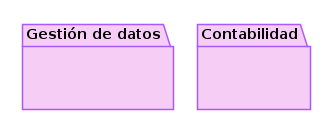
\includegraphics{diagramas/paquetes}
\end{figure}
	
	
\end{document}
